%----------------------------------------------------------------------------
\appendix
%----------------------------------------------------------------------------
\chapter*{\fuggelek}\addcontentsline{toc}{chapter}{\fuggelek}
\setcounter{chapter}{\appendixnumber}
%\setcounter{equation}{0} % a fofejezet-szamlalo az angol ABC 6. betuje (F) lesz
\numberwithin{equation}{section}
\numberwithin{figure}{section}
\numberwithin{lstlisting}{section}
%\numberwithin{tabular}{section}



%----------------------------------------------------------------------------
\section{Példa 1}
\label{sec:example1}
%----------------------------------------------------------------------------

\begin{verbatim}
S! -> S_NP_S_BAR(NP, S_BAR)
[tree] @(?2,?1)

S_BAR -> S_NP_VP(VP, PUNCT)
[tree] S3( *, ?1, ?2)

VP -> VP_VB_NP(VB,NP)
[tree] VP2(?1,?2)

NP -> NP_NN(NN)
[tree] NP1(?1)


NN -> John_NNP
[tree] NNP(John)

NN -> Mary_NNP
[tree] NNP(Mary)

VB -> loves_VBZ
[tree] VBZ(loves)

PUNCT -> punct_PUNCT
[tree] .(.)
\end{verbatim}

\begin{figure}[h]
\centering
\graphicspath{./}
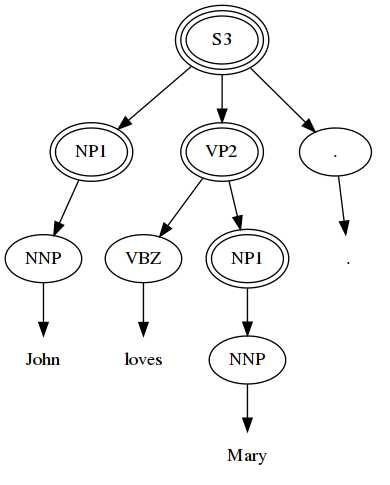
\includegraphics[scale=0.5]{figures/dots/example1.png}
\caption{~\ref{sec:example1}-ben leírt IRTG által generált levezetési fa a \textit{John Loves Mary.} mondat TT-jére.}
\label{fig:example1}
\end{figure}

\begin{verbatim}
@(
	S3( *, VP2( VBZ( loves ),  NP1( NNP( Mary ) ) ), .( . ) ), 
	NP1( NNP( John ) ) 
)
\end{verbatim}

Ebből meg is kapjuk a kívánt TagTree-t.



%----------------------------------------------------------------------------
\section{Példa 2}
\label{sec:example2}
%----------------------------------------------------------------------------

\begin{verbatim}
S! -> NP( DT, JJ, NN )
[tree] NP3(?1,?2,?3)

DT -> the_DT
[tree] DT(the)

JJ -> black_JJ
[tree] NN(black)

VB -> cat_VB
[tree] VB(cat)
\end{verbatim}

Ebből a levezetési fa:
\begin{figure}[h]
\centering
\graphicspath{./}
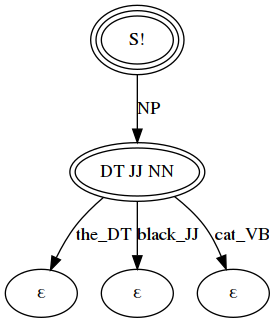
\includegraphics[scale=0.5]{figures/dots/example2.png}
\caption{~\ref{sec:example2}-ben leírt IRTG által generált levezetési fa a \textit{the black cat} szószerkezet TT-jére.}
\label{fig:example2}
\end{figure}

TTA kifejezés (maga a fa): NP3( DT( the ), JJ( black ), NN( cat ) )




%----------------------------------------------------------------------------
\section{Példa 3}
\label{sec:example3}
%----------------------------------------------------------------------------

\begin{verbatim}
S! -> NP_DT_NP_BAR( DT, NP_BAR)
[tree] @(?2,?1)

NP_BAR -> NP_BAR_JJ_NN(JJ,NN)
[tree] NP3(*,?1,?2)

DT -> the_DT
[tree] DT(the)

JJ -> black_JJ
[tree] NN(black)

VB -> cat_VB
[tree] VB(cat)
\end{verbatim}

Ebből a levezetési fa:
\begin{figure}[h]
\centering
\graphicspath{./}
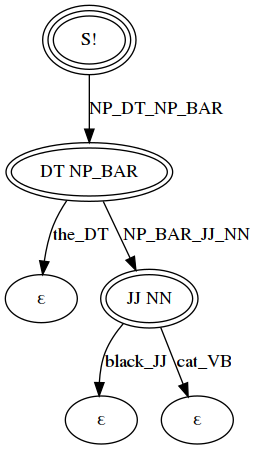
\includegraphics[scale=0.5]{figures/dots/example3.png}
\caption{~\ref{sec:example3}-ban leírt IRTG által generált levezetési fa a \textit{the black cat} szószerkezet TT-jére.}
\label{fig:example3}
\end{figure}

TTA kifejezés: @(  NP3( *, JJ( black ), NN( cat ) ), DT( the ) )




%----------------------------------------------------------------------------
\section{Példa 4}
\label{sec:example4}
%----------------------------------------------------------------------------

\begin{verbatim}
S! -> NP_DT_NP_BAR( DT, NP_BAR)
[tree] @(?2,?1)

NP_BAR -> NP_BAR_JJ_NP_BAR(JJ,NP_BAR)
[tree] @(?2,?1)

NP_BAR -> NP_BAR_JJ_NN(JJ,NN)
[tree] NP4(* ,* ,?1 ,?2)

DT -> this_DT
[tree] DT(this)

JJ -> British_JJ
[tree] JJ(British)

JJ -> indastrial_JJ
[tree] JJ(indastrial)

NN -> conglomerate_NN
[tree] NN(conglomerate)
\end{verbatim}

\begin{figure}[h]
\centering
\graphicspath{./}
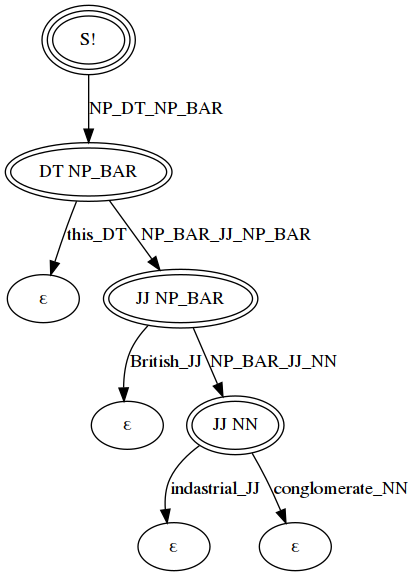
\includegraphics[scale=0.5]{figures/dots/example4.png}
\caption{~\ref{sec:example4}-ben leírt IRTG által generált levezetési fa a \textit{this British indastrial conglomerate} szószerkezet TT-jére.}
\label{fig:example4}
\end{figure}




%----------------------------------------------------------------------------
\section{Példa 5}
\label{sec:example5}
%----------------------------------------------------------------------------

\begin{verbatim}
S! -> root_nsubj_NP_S_BAR(NP, S_BAR)
[ud] merge(
			f_dep(merge("(Root/Root :root r<root> :nsubj (d<dep>))", r_dep(?1))),
	 		?2
	 		)

S_BAR -> S_BAR_VP_PUNCT(VP, PUNCT)
[ud] ?1

VP -> dobj_VB_NP(VB,NP)
[ud] merge(f_dep(merge("(r<root> :dobj (d<dep>))", r_dep(?2))),?1)

NP -> NP_NN(NN)
[ud] ?1


NN -> John_NNP
[ud] "(John<root> / John)"

NN -> Mary_NNP
[ud] "(Mary<root> / Mary)"

VB -> loves_VBZ
[ud] "(loves<root> / loves)"

PUNCT -> punct_PUNCT
[ud] "(punct<root> / punct)"
\end{verbatim}

\begin{figure}[h]
\centering
\graphicspath{./}
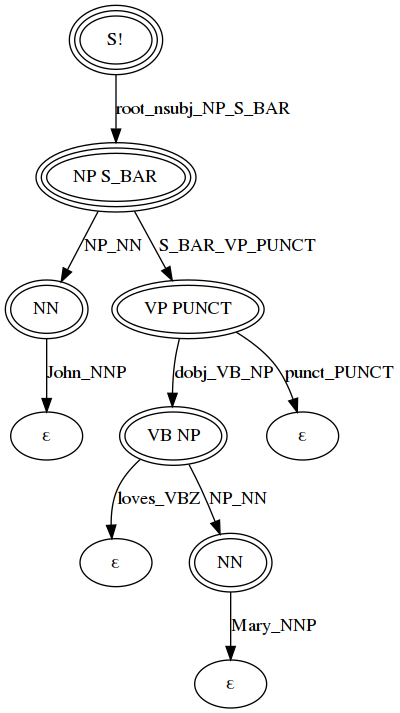
\includegraphics[scale=0.5]{figures/dots/example5_1.png}
\caption{~\ref{sec:example5}-ben leírt IRTG által generált levezetési fa a \textit{John loves Mary.} szószerkezet ud-jét leíró s-graph-ra}
\label{fig:example5.1}
\end{figure}

\begin{figure}[h]
\begin{verbatim}
merge(
	f_dep( merge(
		"(Root/Root :root r<root> :nsubj (d<dep>))",
 		r_dep( "(John<root> / John)" )
		) ),
	 merge(
		f_dep( merge(
					"(r<root> :dobj (d<dep>))", 
					r_dep( "(Mary<root> / Mary)" )
					) ),
 		“(loves<root> / loves)”
		)
	)
\end{verbatim}
\caption{~\ref{sec:example5} ud interpretációjának kimenete}
\label{fig:example6fourlang}
\end{figure}

\begin{figure}[h]
\centering
\graphicspath{./}
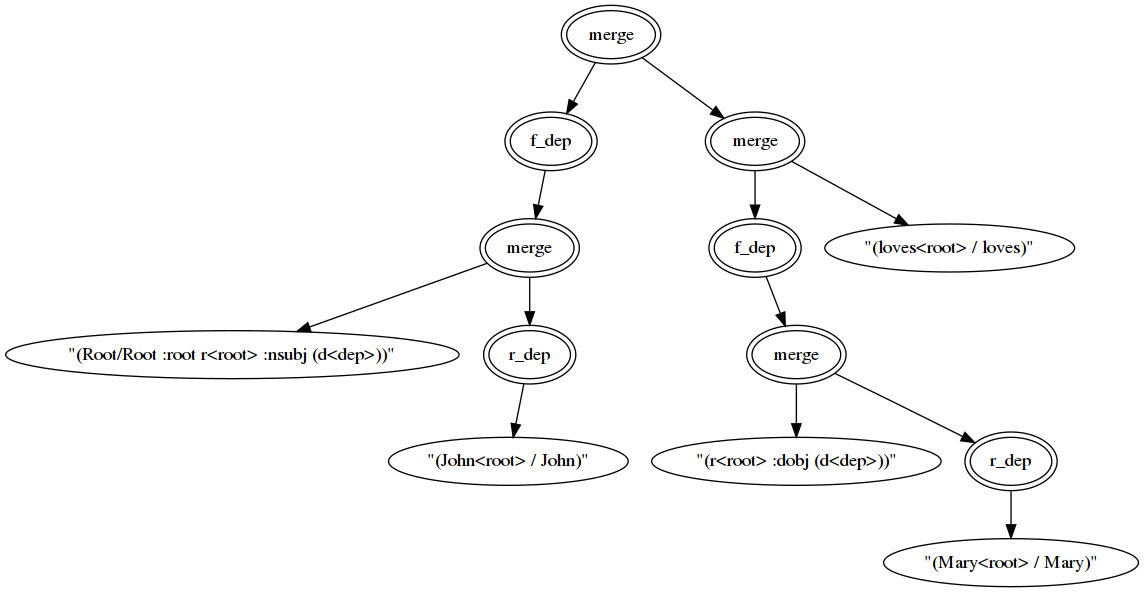
\includegraphics[scale=0.4]{figures/dots/example5_2.png}
\caption{~\ref{sec:example5}-ben leírt IRTG ud interpretációja által generált s-graph kifejezés műveleti fája}
\label{fig:example5.2}
\end{figure}

"(Root/Root :root loves<root>/loves :nsubj (John/John) :dobj (Mary/Mary))"
\begin{figure}[h]
\centering
\graphicspath{./}
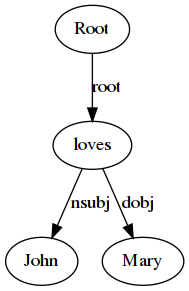
\includegraphics[scale=0.5]{figures/dots/example5_3.png}
\caption{~\ref{sec:example5}-ben leírt IRTG ud interpretációja által generált s-graph kifejezés végeredménye}
\label{fig:example5.3}
\end{figure}




%----------------------------------------------------------------------------
\section{Példa 6}
\label{sec:example6}
%----------------------------------------------------------------------------

\begin{verbatim}
S! -> root_nsubj_NP_S_BAR(NP, S_BAR)
[tree] @(?2,?1)
[ud] merge(
			f_dep(merge("(Root/Root :root r<root> :nsubj (d<dep>))", r_dep(?1))),
			?2
			)
[fourlang] merge(
				f_dep(merge("(Root/Root :root r<root> :1,0 (d<dep>))", r_dep(?1))),
				?2
				)

S_BAR -> S_NP_VP(VP, PUNCT)
[tree] S3( *, ?1, ?2)
[ud] ?1
[fourlang] ?1

VP -> dobj_VB_NP(VB,NP)
[tree] VP2(?1,?2)
[ud] merge(
			f_dep(merge("(r<root> :dobj (d<dep>))", r_dep(?2))),
			?1
			)
[fourlang] merge(
				f_dep(merge("(r<root> :2 (d<dep>))", r_dep(?2))),
				?1
				)

NP -> NP_NN(NN)
[tree] NP1(?1)
[ud] ?1
[fourlang] ?1


NN -> John_NNP
[tree] NNP(John)
[ud] "(John<root> / John)"
[fourlang] "(John<root> / John)"

NN -> Mary_NNP
[tree] NNP(Mary)
[ud] "(Mary<root> / Mary)"
[fourlang] "(Mary<root> / Mary)"

VB -> loves_VBZ
[tree] VBZ(loves)
[ud] "(loves<root> / loves)"
[fourlang] "(loves<root> / loves)"

PUNCT -> punct_PUNCT
[tree] .(.)
[ud] "(punct<root> / punct)"
[fourlang] "(punct<root> / punct)"
\end{verbatim}

\begin{figure}[h]
\centering
\graphicspath{./}
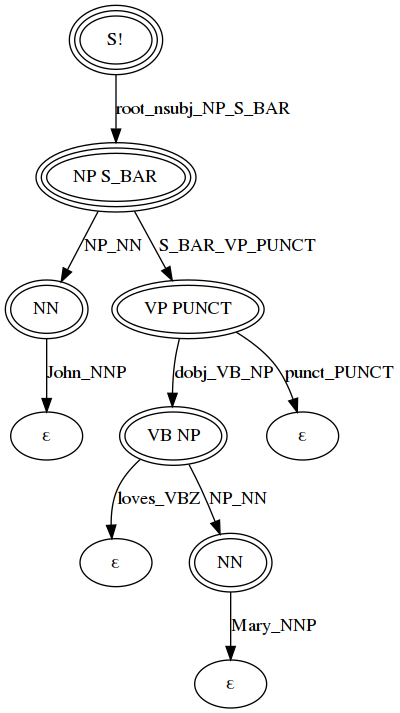
\includegraphics[scale=0.5]{figures/dots/example6_1.png}
\caption{~\ref{sec:example6}-ban leírt IRTG által generált levezetési fa a \textit{John loves Mary.} szószerkezet 4lang-ját leíró s-graph-ra}
\label{fig:example6}
\end{figure}

\begin{figure}[h]
\begin{verbatim}
merge(
	f_dep( 
		merge(
			"(Root/Root :root r<root> :1,0 (d<dep>))",
 			r_dep( 
				"(John<root> / John)" 
				)
			) 
		),
 		merge(
			f_dep( 
					merge(
						"(r<root> :2 (d<dep>))", 
						r_dep( 
							"(Mary<root> / Mary)" 	
							)
						) 
				),
			 “(loves<root> / loves)”
			)
)
\end{verbatim}
\caption{~\ref{sec:example6} fourlang interpretációjának kimenete}
\label{fig:example6fourlang}
\end{figure}

\begin{figure}[h]
\centering
\graphicspath{./}
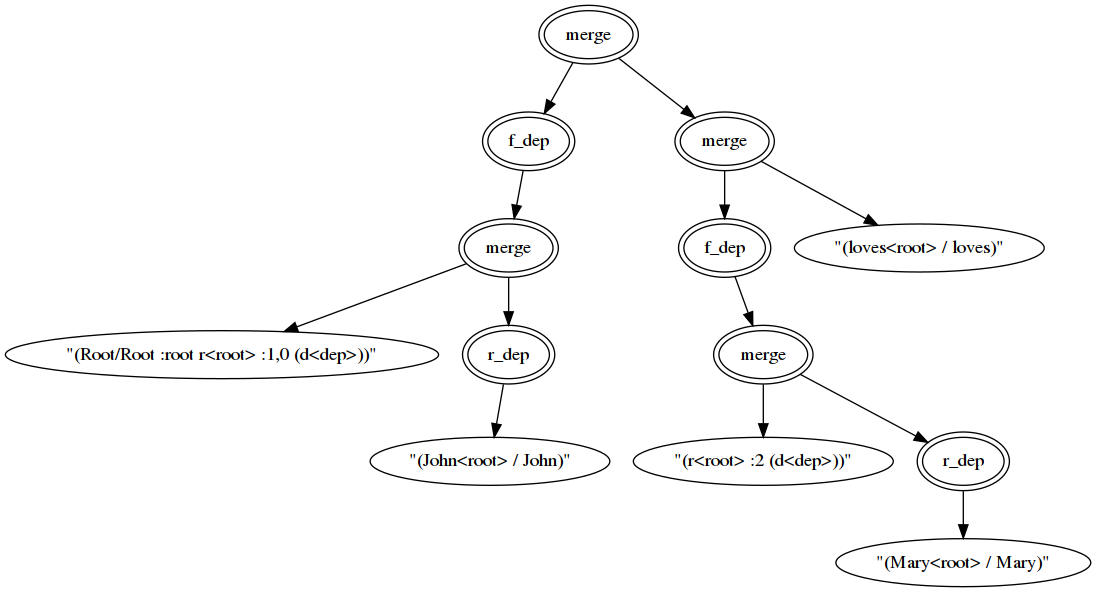
\includegraphics[scale=0.4]{figures/dots/example6_2.png}
\caption{~\ref{sec:example6}-ben leírt IRTG fourlang interpretációja által generált s-graph kifejezés műveleti fája}
\label{fig:example6.2}
\end{figure}

\begin{figure}[h]
\centering
\graphicspath{./}
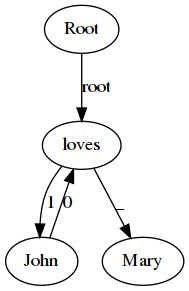
\includegraphics[scale=0.5]{figures/dots/example6_3.png}
\caption{~\ref{sec:example6}-ben leírt IRTG fourlang interpretációja által generált s-graph kifejezés végeredménye}
\label{fig:example6.3}
\end{figure}




%----------------------------------------------------------------------------
\section{Példa 7}
\label{sec:example7}
%----------------------------------------------------------------------------

\begin{verbatim}
//merge start
@(																				
	//merge start
	@(																			
		//graph1
		"( [ Root | | Root ] <root- ( [ r | root ] <nsubj- [ d | dep ] ) )",	
		//graph2
	 	"( [ John | root | John ] )",
	 	//tag of graph1
		dep,							
		//tag of graph2
		root,						
		//tag to forget	
		dep							
	//merge end
	),								
	//merge start
 	@(								
 		//merge start
		@(							
			//graph1
			"([ r | root ] <dobj- [ d | dep ] )", 		
			//graph2	
			"( [ Mary | root | Mary] )",
			//tag of graph1				
			dep,						
			//tag of graph2
			root,					
			//tag to forget	
			dep						
		//merge end
		) ,							
		//graph2
		“( [ loves | root | loves ] )”
	//megre end					
	)								
//merge end
)									
\end{verbatim}



%----------------------------------------------------------------------------
\section{Példa 8}
\label{sec:example8}
%----------------------------------------------------------------------------

\begin{verbatim}


//merge the root of the left graph with root of the right graph
( 
//merge the dep of left graph with the root of the right graph, then we forget dep
( "( [ Root | | Root ] <root- ( [ r | root ] <nsubj- [ d | dep ] ) )" 
>dep@root< 
"( [ John | root | John ] )" X dep ) 

>root@root<

//merge the root of the left graph with root of the right graph
( 

//merge the dep of left graph with the root of the right graph, then we forget dep
( "([ r | root ] <dobj- [ d | dep ] )" 
>dep@root< 	//merge on dep of left graph and root of right graph
"( [ Mary | root | Mary ]  )" X	dep ) 

>root@root<	//merge on root of left graph and root of right graph

“( [ loves | root | loves ]  )” )

)
\end{verbatim}



%----------------------------------------------------------------------------
\section{Példa 9}
\label{sec:example9}
%----------------------------------------------------------------------------



%----------------------------------------------------------------------------
\section{Példa 10}
\label{sec:example10}
%----------------------------------------------------------------------------



%----------------------------------------------------------------------------
\section{Példa 11}
\label{sec:example11}
%----------------------------------------------------------------------------



%----------------------------------------------------------------------------
\section{Példa 11}
\label{sec:example11}
%----------------------------------------------------------------------------



%----------------------------------------------------------------------------
\section{Példa 100}
\label{sec:example100}
%----------------------------------------------------------------------------

\begin{verbatim}
{#A szintaxisban már megoldott, 
hogy nem kell pontosvesszőt rakni, 
ha egyértelműen elkülönülnek a sorok#}
{=
lines, L    :Temp := {|
<$typeB _<$typeM _<$fromB _<$fromM  : '<$pattB <$pattM ' 
-> type(<$asB _<$asM ), pushMode(<$toB _<$toM )<@sc 
|}
linesBasic, LB    :Temp := {|
<$typeB _<$typeM  : '<$pattB |<$pattM ' 
-> pushMode(<$toB _<$toM )<@sc |}

markTypes, MT :List:Temp := [|SLOT;SPEC;REFE;EXTE;PLUS;DECL;DELE;TEXT;TEMP
marks, M	  :List: Temp:= [|$;@;&;*;+;=;x;";|
markModes, MM :List:Temp := [|SLSP;SLSP;REFE;OPER;OPER;OPER;OPER;TEXT;TEMP

markTypesTemp, MTT :List:Temp := [|SLOT;SPEC;TEXT
marksTemp, MT_	  :List: Temp := [|$;@;"
markModesTemp, MMT :List:Temp := [|SLSP;SLSP;TEXT
=}


[= LL :List:Temp 		:= [+ L.fromM 		 :+ [=:List:Temp := [|O;T
[= LLO :List:Temp 		:= [+ LL.0.fromB 	 :+ [=:List:Temp := [|B;O;C
[= LLT :List:Temp 		:= [+ LL.1.fromB 	 :+ [=:List:Temp := [|B;O;C
[= 	LBL :List:Temp 		:= [+ LB.typeB  	 :+ [=:List:Temp := [|BOB;OLB;COB
[= LLOL :List:List:Temp := [+ LLO.iter.typeB :+ [=:List:Temp := [|BOB;OLB;COB
[= LLTL :List:List:Temp := [+ LLT.iter.typeB :+ [=:List:Temp := [|BOB;OLB;COB

[+ 	LBL.iter.pattB 		:+ [=:Iter:Temp := [|{;[;<
[+ LLOL.iter.iter.pattB	:+ [=:Iter:Temp := [|{;[;<
[+ LLTL.iter.iter.pattB	:+ [=:Iter:Temp := [|{;[;<
[+  LBL.iter.toB   		:+ [=:Iter:Temp := [|B;O;C    
[+ LLOL.iter.iter.toB  	:+ [=:Iter:Temp := [|B;O;C
[+ LLTL.iter.iter.toB  	:+ [=:Iter:Temp := [|B;O;C
[+ LLOL.iter.iter.asB  	:+ [=:Iter:Temp := [|BOB;OLB;COB
[+ LLTL.iter.iter.asB  	:+ [=:Iter:Temp := [|BOB;OLB;COB
							
[= 	LBLL :List:List:Temp 	:= [+ LBL.iter.typeM :+ MT
[= LLOLLB :List:List:Temp 	:= [+ LLOL.0.iter.typeM :+ MT
[= LLOLLO :List:List:Temp 	:= [+ LLOL.1.iter.typeM :+ MT
[= LLOLLC :List:List:Temp 	:= [+ LLOL.2.iter.typeM :+ MT
[= LLOLL :List:List:List:Temp 	:= LLOLLB, LLOLLO, LLOLLC
[= LLTLLB :List:List:Temp 	:= [+ LLTL.0.iter.typeM :+ MTT
[= LLTLLO :List:List:Temp 	:= [+ LLTL.1.iter.typeM :+ MTT
[= LLTLLC :List:List:Temp 	:= [+ LLTL.2.iter.typeM :+ MTT
[= LLTLL :List:List:List:Temp 	:=  LLTLLB, LLTLLO, LLTLLC

[+ LBLL.iter.iter.pattM   		:+ M.iter
[+ LLOLL.iter.iter.iter.pattM   :+ M.iter
[+ LBLL.iter.iter.toM     		:+ MM.iter
[+ LLOLL.iter.iter.iter.toM     :+ MM.iter
[+ LLOLL.iter.iter.iter.asM     :+ MT.iter
[+ LLTLL.iter.iter.iter.pattM   :+ MT_.iter
[+ LLTLL.iter.iter.iter.toM     :+ MMT.iter
[+ LLTLL.iter.iter.iter.asM     :+ MTT.iter

{* 
    [# Az alap módba
	<"\\BASIC <@e LBLL : <@e [@e;e;e
	
	[#Az B_OPER módba
	<"\\B_OPER <@e LLOLL.0 : <@e [@e;e
	[#Az O_OPER módba
	<"\\O_OPER <@e LLOLL.1 : <@e [@e;e
	[#Az C_OPER módba
	<"\\C_OPER <@e LLOLL.2 : <@e [@e;e;e
	
	[#Az B_TEMP módba
	<"\\B_OPER <@e LLTLL.0 : <@e [@e;e
	[#Az O_TEMP módba
	<"\\O_OPER <@e LLTLL.1 : <@e [@e;e
	[#Az C_TEMP módba
	<"\\C_OPER <@e LLTLL.2 : <@e [@e;e;e
*}
\end{verbatim}

Ilyen kimenetet ad:

\begin{verbatim}
\\BASIC
BOB_SLOT : '{$' -> pushMode(B_SLSP);
BOB_SPEC : '{@' -> pushMode(B_SLSP);
BOB_REFE : '{&' -> pushMode(B_REFE);
BOB_EXTE : '{*' -> pushMode(B_OPER);
BOB_PLUS : '{+' -> pushMode(B_OPER);
BOB_DECL : '{=' -> pushMode(B_OPER);
BOB_DELE : '{x' -> pushMode(B_OPER);
BOB_TEXT : '{"' -> pushMode(B_TEXT);
BOB_TEMP : '{|' -> pushMode(B_TEMP);
OLB_SLOT : '[$' -> pushMode(O_SLSP);
OLB_SPEC : '[@' -> pushMode(O_SLSP);
OLB_REFE : '[&' -> pushMode(O_REFE);
OLB_EXTE : '[*' -> pushMode(O_OPER);
OLB_PLUS : '[+' -> pushMode(O_OPER);
OLB_DECL : '[=' -> pushMode(O_OPER);
OLB_DELE : '[x' -> pushMode(O_OPER);
OLB_TEXT : '["' -> pushMode(O_TEXT);
OLB_TEMP : '[|' -> pushMode(O_TEMP);
COB_SLOT : '<$' -> pushMode(C_SLSP);
COB_SPEC : '<@' -> pushMode(C_SLSP);
COB_REFE : '<&' -> pushMode(C_REFE);
COB_EXTE : '<*' -> pushMode(C_OPER);
COB_PLUS : '<+' -> pushMode(C_OPER);
COB_DECL : '<=' -> pushMode(C_OPER);
COB_DELE : '<x' -> pushMode(C_OPER);
COB_TEXT : '<"' -> pushMode(C_TEXT);
COB_TEMP : '<|' -> pushMode(C_TEMP);


\\B_OPER
BOB_SLOT_B_O : '{$' ->  type(BOB_SLOT), pushMode(B_SLSP);
BOB_SPEC_B_O : '{@' ->  type(BOB_SPEC), pushMode(B_SLSP);
BOB_REFE_B_O : '{&' ->  type(BOB_REFE), pushMode(B_REFE);
BOB_EXTE_B_O : '{*' ->  type(BOB_EXTE), pushMode(B_OPER);
BOB_PLUS_B_O : '{+' ->  type(BOB_PLUS), pushMode(B_OPER);
BOB_DECL_B_O : '{=' ->  type(BOB_DECL), pushMode(B_OPER);
BOB_DELE_B_O : '{x' ->  type(BOB_DELE), pushMode(B_OPER);
BOB_TEXT_B_O : '{"' ->  type(BOB_TEXT), pushMode(B_TEXT);
BOB_TEMP_B_O : '{|' ->  type(BOB_TEMP), pushMode(B_TEMP);
OLB_SLOT_B_O : '[$' ->  type(OLB_SLOT), pushMode(O_SLSP);
OLB_SPEC_B_O : '[@' ->  type(OLB_SPEC), pushMode(O_SLSP);
OLB_REFE_B_O : '[&' ->  type(OLB_REFE), pushMode(O_REFE);
OLB_EXTE_B_O : '[*' ->  type(OLB_EXTE), pushMode(O_OPER);
OLB_PLUS_B_O : '[+' ->  type(OLB_PLUS), pushMode(O_OPER);
OLB_DECL_B_O : '[=' ->  type(OLB_DECL), pushMode(O_OPER);
OLB_DELE_B_O : '[x' ->  type(OLB_DELE), pushMode(O_OPER);
OLB_TEXT_B_O : '["' ->  type(OLB_TEXT), pushMode(O_TEXT);
OLB_TEMP_B_O : '[|' ->  type(OLB_TEMP), pushMode(O_TEMP);
COB_SLOT_B_O : '<$' ->  type(COB_SLOT), pushMode(C_SLSP);
COB_SPEC_B_O : '<@' ->  type(COB_SPEC), pushMode(C_SLSP);
COB_REFE_B_O : '<&' ->  type(COB_REFE), pushMode(C_REFE);
COB_EXTE_B_O : '<*' ->  type(COB_EXTE), pushMode(C_OPER);
COB_PLUS_B_O : '<+' ->  type(COB_PLUS), pushMode(C_OPER);
COB_DECL_B_O : '<=' ->  type(COB_DECL), pushMode(C_OPER);
COB_DELE_B_O : '<x' ->  type(COB_DELE), pushMode(C_OPER);
COB_TEXT_B_O : '<"' ->  type(COB_TEXT), pushMode(C_TEXT);
COB_TEMP_B_O : '<|' ->  type(COB_TEMP), pushMode(C_TEMP);

\\O_OPER
BOB_SLOT_O_O : '{$' ->  type(BOB_SLOT), pushMode(B_SLSP);
BOB_SPEC_O_O : '{@' ->  type(BOB_SPEC), pushMode(B_SLSP);
BOB_REFE_O_O : '{&' ->  type(BOB_REFE), pushMode(B_REFE);
BOB_EXTE_O_O : '{*' ->  type(BOB_EXTE), pushMode(B_OPER);
BOB_PLUS_O_O : '{+' ->  type(BOB_PLUS), pushMode(B_OPER);
BOB_DECL_O_O : '{=' ->  type(BOB_DECL), pushMode(B_OPER);
BOB_DELE_O_O : '{x' ->  type(BOB_DELE), pushMode(B_OPER);
BOB_TEXT_O_O : '{"' ->  type(BOB_TEXT), pushMode(B_TEXT);
BOB_TEMP_O_O : '{|' ->  type(BOB_TEMP), pushMode(B_TEMP);
OLB_SLOT_O_O : '[$' ->  type(OLB_SLOT), pushMode(O_SLSP);
OLB_SPEC_O_O : '[@' ->  type(OLB_SPEC), pushMode(O_SLSP);
OLB_REFE_O_O : '[&' ->  type(OLB_REFE), pushMode(O_REFE);
OLB_EXTE_O_O : '[*' ->  type(OLB_EXTE), pushMode(O_OPER);
OLB_PLUS_O_O : '[+' ->  type(OLB_PLUS), pushMode(O_OPER);
OLB_DECL_O_O : '[=' ->  type(OLB_DECL), pushMode(O_OPER);
OLB_DELE_O_O : '[x' ->  type(OLB_DELE), pushMode(O_OPER);
OLB_TEXT_O_O : '["' ->  type(OLB_TEXT), pushMode(O_TEXT);
OLB_TEMP_O_O : '[|' ->  type(OLB_TEMP), pushMode(O_TEMP);
COB_SLOT_O_O : '<$' ->  type(COB_SLOT), pushMode(C_SLSP);
COB_SPEC_O_O : '<@' ->  type(COB_SPEC), pushMode(C_SLSP);
COB_REFE_O_O : '<&' ->  type(COB_REFE), pushMode(C_REFE);
COB_EXTE_O_O : '<*' ->  type(COB_EXTE), pushMode(C_OPER);
COB_PLUS_O_O : '<+' ->  type(COB_PLUS), pushMode(C_OPER);
COB_DECL_O_O : '<=' ->  type(COB_DECL), pushMode(C_OPER);
COB_DELE_O_O : '<x' ->  type(COB_DELE), pushMode(C_OPER);
COB_TEXT_O_O : '<"' ->  type(COB_TEXT), pushMode(C_TEXT);
COB_TEMP_O_O : '<|' ->  type(COB_TEMP), pushMode(C_TEMP);

\\C_OPER
BOB_SLOT_C_O : '{$' ->  type(BOB_SLOT), pushMode(B_SLSP);
BOB_SPEC_C_O : '{@' ->  type(BOB_SPEC), pushMode(B_SLSP);
BOB_REFE_C_O : '{&' ->  type(BOB_REFE), pushMode(B_REFE);
BOB_EXTE_C_O : '{*' ->  type(BOB_EXTE), pushMode(B_OPER);
BOB_PLUS_C_O : '{+' ->  type(BOB_PLUS), pushMode(B_OPER);
BOB_DECL_C_O : '{=' ->  type(BOB_DECL), pushMode(B_OPER);
BOB_DELE_C_O : '{x' ->  type(BOB_DELE), pushMode(B_OPER);
BOB_TEXT_C_O : '{"' ->  type(BOB_TEXT), pushMode(B_TEXT);
BOB_TEMP_C_O : '{|' ->  type(BOB_TEMP), pushMode(B_TEMP);
OLB_SLOT_C_O : '[$' ->  type(OLB_SLOT), pushMode(O_SLSP);
OLB_SPEC_C_O : '[@' ->  type(OLB_SPEC), pushMode(O_SLSP);
OLB_REFE_C_O : '[&' ->  type(OLB_REFE), pushMode(O_REFE);
OLB_EXTE_C_O : '[*' ->  type(OLB_EXTE), pushMode(O_OPER);
OLB_PLUS_C_O : '[+' ->  type(OLB_PLUS), pushMode(O_OPER);
OLB_DECL_C_O : '[=' ->  type(OLB_DECL), pushMode(O_OPER);
OLB_DELE_C_O : '[x' ->  type(OLB_DELE), pushMode(O_OPER);
OLB_TEXT_C_O : '["' ->  type(OLB_TEXT), pushMode(O_TEXT);
OLB_TEMP_C_O : '[|' ->  type(OLB_TEMP), pushMode(O_TEMP);
COB_SLOT_C_O : '<$' ->  type(COB_SLOT), pushMode(C_SLSP);
COB_SPEC_C_O : '<@' ->  type(COB_SPEC), pushMode(C_SLSP);
COB_REFE_C_O : '<&' ->  type(COB_REFE), pushMode(C_REFE);
COB_EXTE_C_O : '<*' ->  type(COB_EXTE), pushMode(C_OPER);
COB_PLUS_C_O : '<+' ->  type(COB_PLUS), pushMode(C_OPER);
COB_DECL_C_O : '<=' ->  type(COB_DECL), pushMode(C_OPER);
COB_DELE_C_O : '<x' ->  type(COB_DELE), pushMode(C_OPER);
COB_TEXT_C_O : '<"' ->  type(COB_TEXT), pushMode(C_TEXT);
COB_TEMP_C_O : '<|' ->  type(COB_TEMP), pushMode(C_TEMP);


\\B_TEMP
BOB_SLOT_B_T : '{$' -> type(BOB_SLOT), pushMode(B_SLSP);
BOB_SPEC_B_T : '{@' -> type(BOB_SPEC), pushMode(B_SLSP);
BOB_TEXT_B_T : '{"' -> type(BOB_TEXT), pushMode(B_TEXT);
OLB_SLOT_B_T : '[$' -> type(OLB_SLOT), pushMode(O_SLSP);
OLB_SPEC_B_T : '[@' -> type(OLB_SPEC), pushMode(O_SLSP);
OLB_TEXT_B_T : '["' -> type(OLB_TEXT), pushMode(O_TEXT);
COB_SLOT_B_T : '<$' -> type(COB_SLOT), pushMode(C_SLSP);
COB_SPEC_B_T : '<@' -> type(COB_SPEC), pushMode(C_SLSP);
COB_TEXT_B_T : '<"' -> type(COB_TEXT), pushMode(C_TEXT);

\\O_TEMP
BOB_SLOT_O_T : '{$' -> type(BOB_SLOT), pushMode(B_SLSP);
BOB_SPEC_O_T : '{@' -> type(BOB_SPEC), pushMode(B_SLSP);
BOB_TEXT_O_T : '{"' -> type(BOB_TEXT), pushMode(B_TEXT);
OLB_SLOT_O_T : '[$' -> type(OLB_SLOT), pushMode(O_SLSP);
OLB_SPEC_O_T : '[@' -> type(OLB_SPEC), pushMode(O_SLSP);
OLB_TEXT_O_T : '["' -> type(OLB_TEXT), pushMode(O_TEXT);
COB_SLOT_O_T : '<$' -> type(COB_SLOT), pushMode(C_SLSP);
COB_SPEC_O_T : '<@' -> type(COB_SPEC), pushMode(C_SLSP);
COB_TEXT_O_T : '<"' -> type(COB_TEXT), pushMode(C_TEXT);

\\C_TEMP
BOB_SLOT_C_T : '{$' -> type(BOB_SLOT), pushMode(B_SLSP);
BOB_SPEC_C_T : '{@' -> type(BOB_SPEC), pushMode(B_SLSP);
BOB_TEXT_C_T : '{"' -> type(BOB_TEXT), pushMode(B_TEXT);
OLB_SLOT_C_T : '[$' -> type(OLB_SLOT), pushMode(O_SLSP);
OLB_SPEC_C_T : '[@' -> type(OLB_SPEC), pushMode(O_SLSP);
OLB_TEXT_C_T : '["' -> type(OLB_TEXT), pushMode(O_TEXT);
COB_SLOT_C_T : '<$' -> type(COB_SLOT), pushMode(C_SLSP);
COB_SPEC_C_T : '<@' -> type(COB_SPEC), pushMode(C_SLSP);
COB_TEXT_C_T : '<"' -> type(COB_TEXT), pushMode(C_TEXT);
\end{verbatim}

Tehát a szűk felére esett össze a szöveg.
Ha a markTypes, marks, markModes, markTypesTemp, marksTemp, markModesTemp változókat a felhasználások helyén deklaráltuk volna,
és a lines és linesBasic Temp-eket pedig egysorban deklaráltuk volna, akkor már harmad annyi sorban is megoldhattuk volna.
Még így is maradtak a kódban összevonható sorok.
Persze a kimenet is szebben lenne tagolva, ha minden TEXT sor végére beszúrtunk volna egy entert.
Az Iter segítségével ez sem lett volna olyan nehéz.